\documentclass[]{article}
\usepackage[utf8]{inputenc}
\usepackage{polski}
\usepackage{listings}
\usepackage[usenames,dvipsnames]{xcolor}
\usepackage{geometry}
\usepackage{subcaption}
\usepackage{graphicx}
\usepackage{amsmath}
\usepackage{amssymb}
\usepackage{enumerate}
\usepackage[font=small]{caption}
\DeclareGraphicsExtensions{.png}
\graphicspath{ {./} }
\geometry{
	a4paper,
	left=25mm,
	right = 25mm,
	top=25mm,
}
%%\hyphenchar\font=-1

\title{
	Sprawozdanie \\
	\large 
	Obliczenia naukowe - lista 3}
\author{Kamil Król}
\date{244949}


\begin{document}
	
	\maketitle
	
	\section*{Zadanie 1}
	Celem tego zadania było napisanie funkcji w języku Julia, która rozwiązuje równanie $f(x) = 0$ metodą bisekcji oraz opis tej metody.\\
	\textbf{Dane:}
	\begin{enumerate}[]
		\item $f(x)$ -- funkcja ciągła w przedziale $[a,b]$,
		\item $[a,b]$ -- przedział początkowy, w którym szukamy zera funkcji $f$ i który spełnia warunek $f(a)f(b)< 0$,
		\item $\epsilon, \delta$ -- dokładności obliczeń.
	\end{enumerate}
	\textbf{Opis:}\\
	Zanim przystąpimy do opisu tej metody przypomnijmy twierdzenie Darboux. Mówi ono, że jeżeli funkcja $f$ jest ciągła na przedziale $[a,b]$ i $f(a)f(b)<0$ czyli wartości funkcji $f$ na końcach przedziału mają różne znaki, to istnieje taki punkt $c\in[a,b]$, dla którego $f(c)=0$. Metoda bisekcji korzysta właśnie z tego twierdzenia do znalezienia miejsc zerowych funkcji $f$. Stąd biorą się wymagania co do danych tzn. funkcja $f$ ciagła na $[a,b]$ oraz warunek $f(a)f(b)< 0$. Metoda bisekcji polega na iteracyjnym połowieniu przedziału początkowego. Początkowy przedział $[a,b]$ spełnia warunek $f(a)f(b)< 0$ z warunków początkowych. Następnie ten przedział jest połowiony. W wyniku podziału otrzymujemy przedziały $[a,c]$ oraz $[c,b]$ gdzie $c$ jest środkiem przedziału $[a,b]$. Teraz musimy sprawdzić, który z tych przedziałów spełnia warunek mówiący o tym, że wartości funkcji $f$ na jego końcach mają różne znaki. Wybieramy przedział spełniający ten warunek i dla niego powtarzamy tę procedurę. Kończymy w momencie kiedy znajdziemy zero funkcji z zadaną dokładnością tj. $|f(c)|<\epsilon$ lub kiedy szerokość przedziału, w którym szukamy zera jest dostatecznie mała tzn. $b-a<\delta$.\\
	\textbf{Uwagi implementacyjne:}\\
	Na początek zastanówmy się w jaki sposób można obliczyć środek przedziału $[a,b]$. Najprostszą metodą wydaje się obliczenie średniej arytmetycznej tj. $c=\frac{a+b}{2}$. Z numerycznego punktu widzenia jest to metoda ryzykowna, gdyż w pewnych przypadkach moglibyśmy otrzymać środek przedziału $c$ nienależący do przedziału $[a,b]$. Dlatego środek przedziału obliczamy ze wzoru: $c = a + \frac{b-a}{2}$. Kolejnym niebezpieczeństwem jest sprawdzanie warunku $f(*)f(c)< 0$. Mnożenie po lewej stronie nierówności może w rezultacie dać nadmiar lub niedomiar. Można go uniknąć poprzez jawne sprawdzenie znaków $f(*)$ i $f(c)$ tj. $sign(f(*)) \neq sign(f(c))$.
	
	
	\clearpage
	
	\section*{Zadanie 2}
	
	Celem tego zadania było napisanie funkcji w języku Julia, która rozwiązuje równanie $f(x) = 0$ metodą Newtona oraz opis tej metody. Metoda Newtona nazywana jest też metodą stycznych.\\
	\textbf{Dane:}
	\begin{enumerate}[]
		\item $[a,b]$ -- przedział na którym wykonywać będziemy obliczenia,
		\item $f(x)$, $f'(x)$  -- funkcja $f$ należąca do klasy $C^2[a,b]$ oraz pochodna funkcji $f$
		\item $x_0$ -- przybliżenie początkowe,
		\item $\epsilon, \delta$ -- dokładności obliczeń,
		\item \texttt{maxit} -- maksymalna dopuszczalna liczba iteracji.
	\end{enumerate}
	\textbf{Opis:}\\
	Dodatkowym założeniem jest to, że szukamy pierwiastka $r$ dla którego $f'(r)\ne0$, tzn. pierwiastek $r$ jest pierwiastkiem jednokrotnym. Metoda Newtona opiera się na linearyzacji funkcji (zastąpieniu jej funkcją liniową) przez użycie jej rozwinięcia w szereg Taylora.
	$$f(x) = f(x_n ) + f'(x_n )(x-x_n) + O((x-x_n )^2)\text{ -- rozwinięcie w szereg Taylora}$$
	$$f(x)\approx f(x_n ) + f'(x_n )(x-x_n) \text{ -- linearyzacja}$$
	Mamy zatem równianie $f(x_n ) + f'(x_n )(x_{n+1}-x_n) = 0$ co po przekształceniu daje wzór rekurencyjny $x_{n+1} = x_n - \dfrac{f(x_n)}{f'(x_n)}$. Jest to wzór na kolejne przybliżenia zera funkcji. Widać, też dlaczego pojawia się założenie o tym że $f'(r)\ne0$ -- dzielilibyśmy wtedy przez 0. Zauważmy teraz, że styczna do wykresu funkcji $f$ w punkcie $x_n$ przecina oś OX w punkcie $(x_{n+1},0)$. Stąd właśnie bierze się alternatywna nazwa metody Newtona - metoda stycznych.
	\begin{figure}[!htbp]
		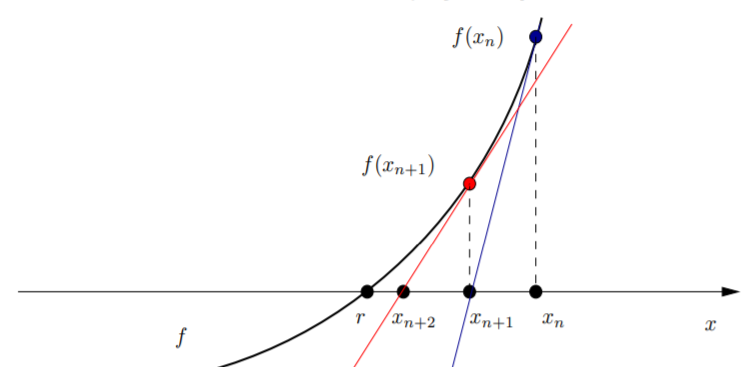
\includegraphics[scale=0.7]{newton}
		\centering
		\caption{Interpretacja graficzna metody Newtona -- grafika z wykładu}
	\end{figure}

	Na początku algorytmu następuje sprawdzenie czy wartość $f(x_0)$ jest dostatecznie bliska zeru tzn. $|f(x_0)|<\epsilon$. Jeśli tak to kończymy pracę algorytmu i zwracamy wynik. W przeciwnym wypadku przystępujemy do następnego kroku i sprawdzamy czy wartość pochodnej nie jest zbyt bliska zeru tj. $|f'(x_0)|<\epsilon$. Jeśli by się tak stało dalsze obliczenia nie miałyby sensu. Następnie używając podanego wcześniej wzoru rekurencyjnego wyliczamy iteracyjnie kolejne przybliżenia pierwiastka. Robimy to dopóki nie osiągniemy pożądanej dokładności tj. $|f(x_n)|<\epsilon$ lub nie otrzymamy dostatecznie bliskich sobie przybliżeń tj. $|x_n-x_{n-1}|<\delta$. Jeśli nie uda się spełnić tych warunków w dopuszczalnej liczbie iteracji przerywamy obliczenia. Szczególną sytuacją kiedy nie uda nam się spełnić tych warunków jest to kiedy metoda Newtona okazuje się rozbieżna dla zadanego $x_0$. Inaczej mówiąc, może się tak zdażyć, że dla zadanego przybliżenia początkowego $x_0$ metoda Newtona nie jest zbieżna. Widać zatem, że nie jest to metoda zbieżna globalnie. Dlatego właśnie stosuje się ją często w połączeniu z inna metodą zbieżną globalnie.
	Metoda Newtona jest szybsza niż metoda bisekcji, ponieważ ma kwadratowy współczynnik zbieżności.
	\\
	%\textbf{Uwagi implementacyjne:}\\

	\section*{Zadanie 3} 
	
	Celem tego zadania było napisanie funkcji w języku Julia, która rozwiązuje równanie $f(x) = 0$ metodą siecznych oraz opis tej metody.\\
	\textbf{Dane:}
	\begin{enumerate}[]
		\item $[a,b]$ -- przedział na którym wykonywać będziemy obliczenia,
		\item $f(x)$ -- funkcja $f$ należąca do klasy $C^2[a,b]$,
		\item $x_0$, $x_1$ -- przybliżenia początkowe,
		\item $\epsilon, \delta$ -- dokładności obliczeń,
		\item \texttt{maxit} -- maksymalna dopuszczalna liczba iteracji.
	\end{enumerate}
	\textbf{Opis:}\\
	Dodatkowym założeniem jest to, że szukamy pierwiastka $r$ dla którego $f'(r)\ne0$, tzn. pierwiastek $r$ jest pierwiastkiem jednokrotnym -- tak samo jak dla metody Newtona.
	Zanim przystąpimy do opisu metody siecznych przyjrzyjmy się jeszcze raz metodzie Newtona. Wadą metody Newtona jest konieczność obliczenia pochodnej funkcji $f$. Metoda siecznych różni się od metody Newtona tym, że zamiast obliczać wartość $f'(x_n)$, aproksymujemy ją używając następującej formuły: $f'(x_n) \approx \dfrac{f(x_n)-f(x_{n-1})}{x_n-x_{n-1}}$. Przypomnijmy, że w metodzie Newtona kolejne przybliżenia otrzymywaliśmy ze wzoru rekurencyjnego: $x_{n+1} = x_n - \dfrac{f(x_n)}{f'(x_n)}$. Kiedy pochodną funkcji $f$ zastąpimy powyższym przybliżeniem otrzymujemy wzór: $x_{n+1} := x_n - f(x_n)\dfrac{x_n-x_{n-1}}{f(x_n)-f(x_{n-1})}$. Widzimy zatem, że metoda siecznych jest modyfikacją meotdy Newtona, która \textit{ucieka} od liczenia wartości pochodnej funkcji $f$. Kiedy przyjrzymy się dokładniej otrzymanemu wzorowi rekurencyjnemu widzimy, że pojawiła się potrzeba znajomości dwóch poprzednich wartości $x$. Dlatego właśnie w danych pojawia się $x_0$, $x_1$. Warunkiem końcowym jest znalezienie pierwiastka z pożądaną dokładnością tj. $|f(x_n)|<\epsilon$ lub otrzymanie dostatecznie bliskich sobie przybliżeń tj. $|x_n-x_{n-1}|<\delta$. (Warunki takie same jak dla metody Newtona). Może się zdarzyć, że dla zadanych przybliżeń początkowych metoda siecznych nie jest zbieżna, ponieważ metoda siecznych nie jest zbieżna globalnie. Zatem w przypadku nieosiągnięcia warunków końcowych w maksymalnej dopuszczalnej liczbie iteracji zwracany jest błąd. Współczynnik zbieżności metody siecznych wynosi $\alpha = \frac{1+\sqrt{5}}{2}\approx1.618$. 
	Interpretacja graficzna tej metody wygląda w następujący sposób. Każne kolejne przybliżenie pierwiastka $x_{n+2}$ to przecięcie siecznej poprowadzonej przez punkty $(x_n$, $f(x_n))$ i $(x_{n+1}$, $f(x_{n+1}))$, gdzie $x_n$ i $x_{n+1}$ to dwa poprzednie przybliżenia, z osią OX. Poniżej grafika.
	\begin{figure}[!htbp]
		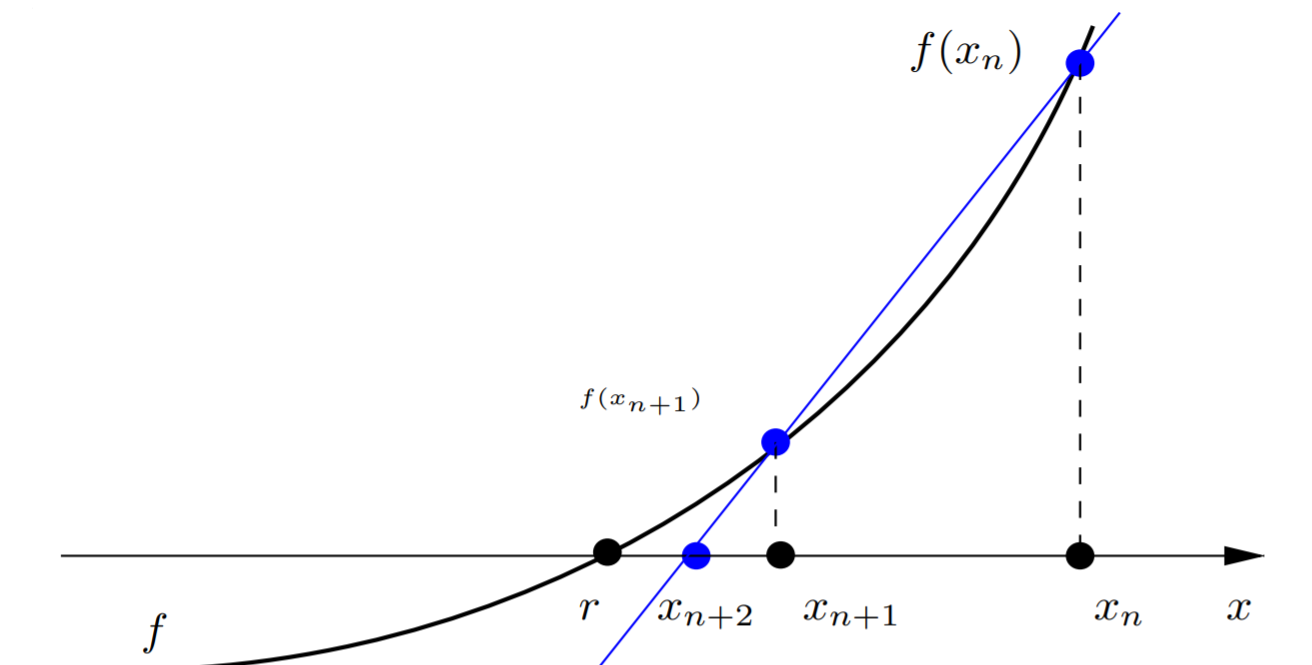
\includegraphics[scale=0.59]{secant}
		\centering
		\caption{Interpretacja graficzna metody siecznych -- grafika z wykładu}
	\end{figure}
	\clearpage

	\noindent\textbf{Uwagi implementacyjne:}\\
	W implementacji tej metody dodano warunek mówiący, że kolejne wartości bezwzględne wartości funkcji tworzą ciąg nierosnący tzn. $|f(x_n)| \leq |f(x_{n+1})|$. W przypadku kiedy trafią się wartości $x_n$ i $x_{n+1}$, które nie spełniają tego warunku, są one ze sobą zamieniane.
	
	
	
	
	\section*{Zadanie 4}

	Celem zadania było wyznaczenie pierwiastków równania $\sin{x}-(\frac{1}{2}x)^2 = 0$ używając wcześniej zaimplementowanych metod:
	\begin{enumerate}[(a)]
		\item metody bisekcji (z przedziałem początkowym $[1.5, 2.0]$),
		\item metody Newtona (z przybliżeniem początkowym $x_0 = 1.5$),  
		\item metody siecznych (z przybliżeniami początkowymi $x_0 = 1.0$ i $x_1 = 2.0$).
	\end{enumerate}
	Dla wszystkich metod dokładności były wspólne tj. $\delta = \epsilon = \frac{1}{2}10^{-5}$. Za maksymalną liczbę iteracji przyjąłem 40. Zacząłem od obliczenia pochodnej funkcji $f$, $f'(x) = \cos{x} - \frac{1}{2}x$ potrzebnej w metodzie Newtona. Wyniki działania programów znajdują się w tabeli poniżej.
	
	\begin{table}[h!]
		\centering
		\label{tab:table1}
		\begin{tabular}{|c|c|c|c|}
			\hline
			metoda & wartość pierwiastka - $r$ & wartość funkcji w punkcie $r$ - $f(r)$ & liczba iteracji \\ \hline
			metoda bisekcji & 1.9337539672851562 & -2.7027680138402843e-7 & 16 \\ \hline
			metoda Newtona & 1.933753779789742 & -2.2423316314856834e-8 & 4 \\ \hline
			metoda siecznych & 1.933753644474301 & 1.564525129449379e-7 & 4 \\ \hline
		\end{tabular}
	\end{table}
	
	Widać, że różnica w ilości wykonanych iteracji między metodą bisekcji a dwoma pozostałymi jest znaczna. Metoda bisekcji okazała się najwolniejsza. Metody Newtona i siecznych okazały się w tym przypadku porównywalne jeśli chodzi o ilość iteracji potrzebną do osiągnięcia zadanej dokładności. Wyniki eksperymentu mają odzwierciedlenie w teorii. Współczynnik zbieżności dla metody siecznych wynosi $1$ (zbieżność liniowa), dla metody Newtona $2$ (zbieżność kwadratowa), a dla metody siecznych $\approx1.62$.
	
	\clearpage
	
	\section*{Zadanie 5}
	Celem zadania było użycie metody bisekcji do znalezienia, wartości zmiennej $x$, dla której przecinają się wykresy funkcji $y=3x$ oraz $y=e^x$. Zadane dokładności wynosiły $\delta = \epsilon = 10^{-4}$. Zadanie można sprowadzić do problemu rozwiązania równania $e^x - 3x = 0$ lub równoważnie znalezienia miejsc zerowych funkcji $f(x) = e^x - 3x$. Pierwszą rzeczą jaką należało wykonać to dobrać przedział lub przedziały początkowe. Wiemy, że metoda bisekcji wymaga takiego przedziału, że wartości funkcji w jego końcach mają różny znak. W celu wyznaczenia przedziałów początkowych posłużyłem się poniższymi wykresami.
	
	\begin{figure}[!htbp]
		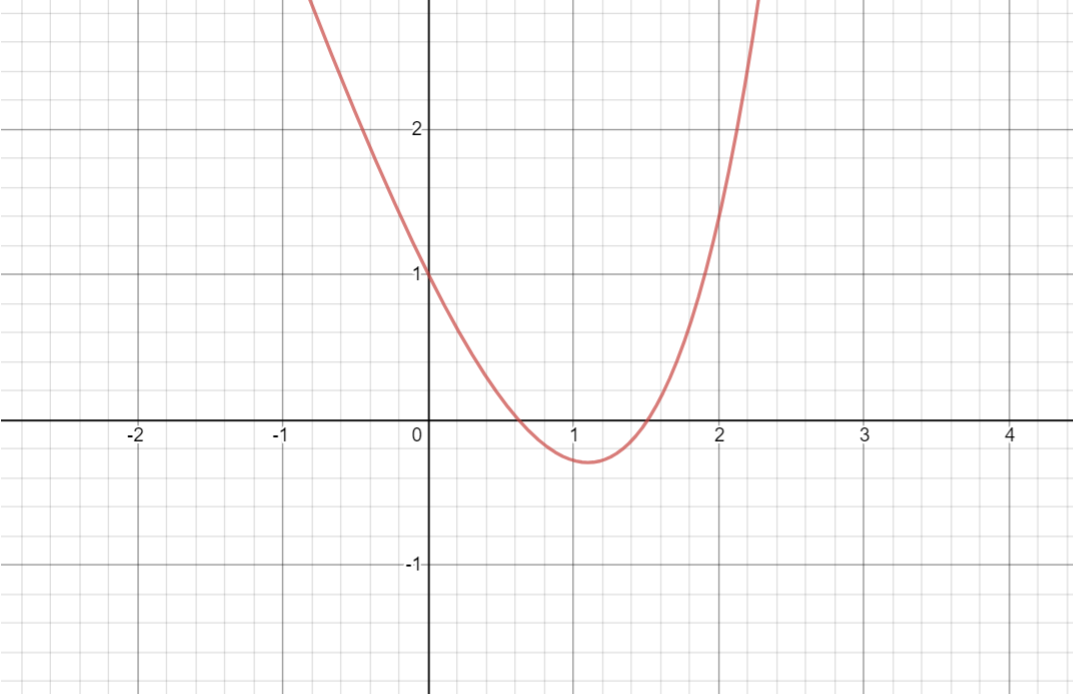
\includegraphics[width=\textwidth]{task5plot}
		\centering
		\caption{Wykres funkcji $f(x) = e^x - 3x$}
	\end{figure}
	
%	\begin{figure}[!htbp]
%		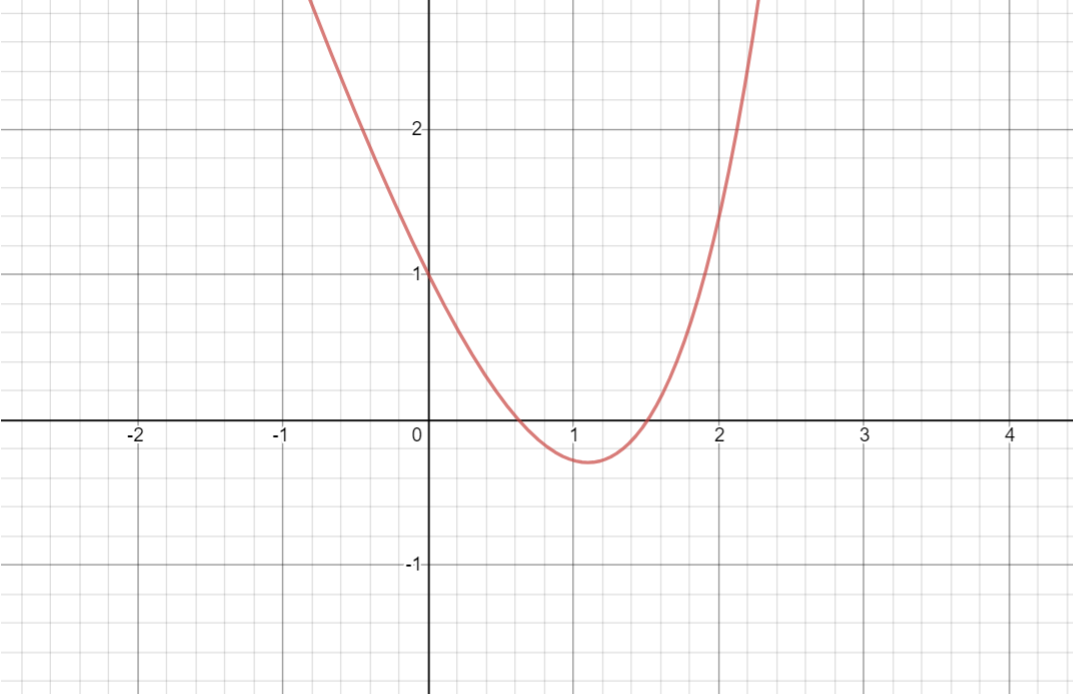
\includegraphics[height=0.38\textheight]{task5plot}
%		\centering
%		\caption{Wykres funkcji $f(x) = e^x - 3x$}
%	\end{figure}
%	\begin{figure}[!htbp]
%		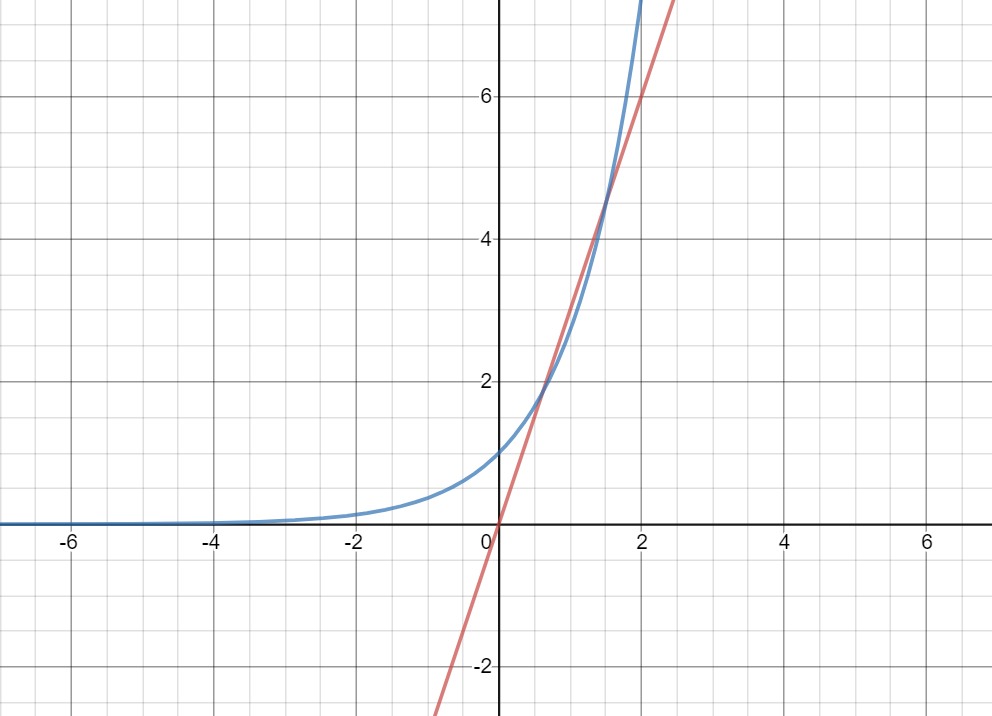
\includegraphics[height=0.36\textheight]{3xexplot}
%		\centering
%		\caption{Wykresy funkcji $e^x$ i $3x$}
%	\end{figure}

	Patrząc na wykresy wybrałem przedziały [0,1] oraz [1,2]. Oba z nich spełniają wymagania metody bisekcji. Znalezione pierwiastki to $x_1=0.619140625$ oraz $x_2=1.5120849609375$ co pokrywa się z tym co sugeruje wykres.
	
	
	\begin{table}[!h]
		\centering
		\label{tab:table1}
		\begin{tabular}{c|c|c}
			
			 & $x_1$ & $x_2$ \\ \hline
			Wartość pierwiastka $r$ &  0.619140625 & 1.5120849609375 \\ 
			Wartość funkcji $f(r)$ & -9.066320343276146e-5 & -7.618578602741621e-5  \\ 
			Liczba iteracji & 9 & 13 \\
			Przedział & [0,1] & [1,2] \\
		\end{tabular}
	\end{table}

	Widać, że oba pierwiastki występują dość blisko siebie oraz fakt, że znacznym ułatwieniem w znaleznieniu przedziałów początkowych była znajomość przebiegu funkcji $f$. Na wykresie od razu widać było, że powinniśmy się spodziewać dokładnie dwóch miejsc zerowych oraz gdzie się ich spodziewać. Bez pomocy jaką była znajomość przebiegu funkcji $f$ nie wiedzielibyśmy nawet ilu miejsc zerowych powinniśmy się spodziewać. Innym wnioskiem jest fakt, że znalezione miejsce zerowe zależy od wybranego przedziału początkowego. Ogólniejszym wnioskiem jest to, że bez dobrej znajomości przebiegu funkcji metoda bisekcji może być problematyczna do zastosowania. 

	\clearpage
	
	\section*{Zadanie 6}
	
	Celem zadania było znalezienie miejsc zerowych funkcji $f_1(x)=e^{1-x}-1$ oraz $f_2(x)=xe^{-x}$ przy pomocy metod bisekcji, stycznych oraz siecznych z dokładnością obliczeń $\delta=\epsilon=10^{-5}$. Przyblizenia początkowe oraz przedział początkowy należało dobrać samodzielnie.\\
	W celu wzynaczenie danych startowych narysowałem wykresy obu funkcji. Wykresy poniżej.

	\begin{figure}[!htbp]
		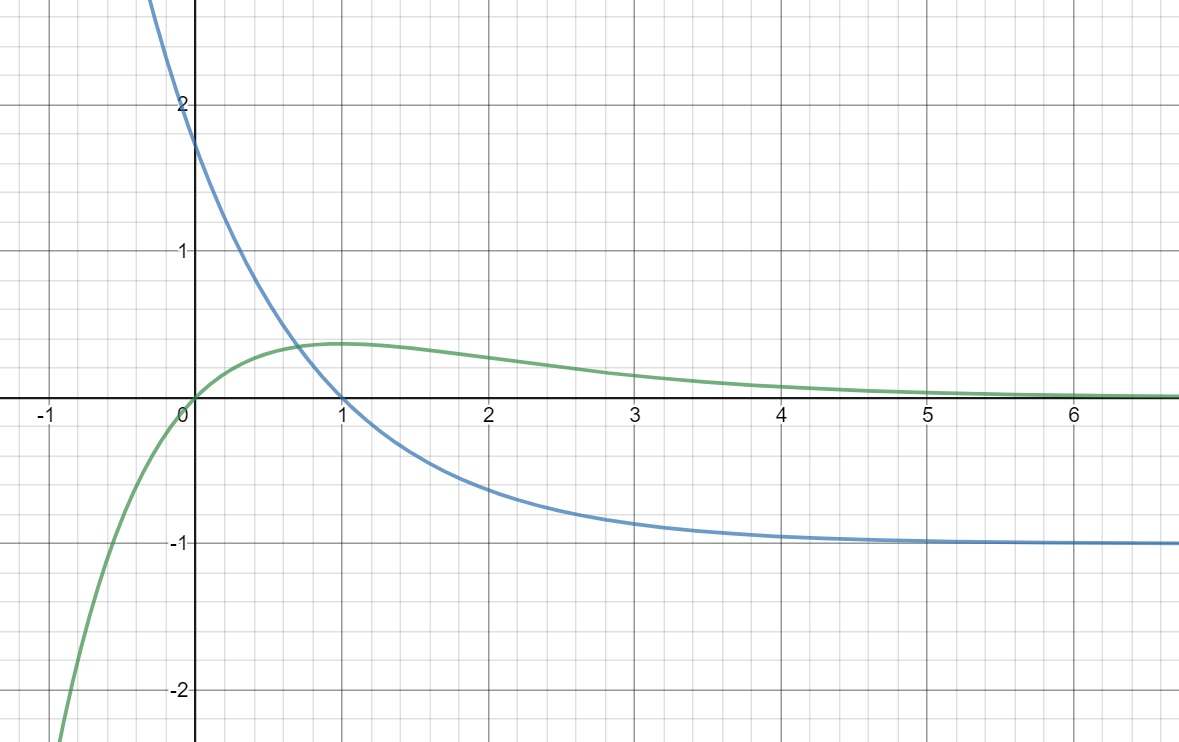
\includegraphics[width=\textwidth]{e1-x-1andxe-x.png}
		\centering
		\caption{Wykresy funkcji $f_1(x)=e^{1-x}-1$ oraz $f_2(x)=xe^{-x}$ narysowane w programie Desmos.}
	\end{figure}
	\noindent\textbf{Metoda bisekcji}

	\noindent Widać, że $f_1$ ma tylko jedno miejsce zerowe i jest nim $x=1$. Na podstawie wykresu wybrałem przedziały startowe dla metody bisekcji dla funkcji $f_1$.
	
	\begin{table}[!h]
		\centering
		\label{tab:table1}
		\begin{tabular}{|c|c|c|c|}
			\hline
			przedział & pierwiastek - $r$ & $f_1(r)$ & liczba potrzebych iteracji\\
			\hline
			[0.0, 2.0] & 1.0 & 0.0 & 1 \\ \hline
			[0.4, 2.4] & 1.000006103515625 & -6.103496998477453e-6 & 16 \\ \hline
			[-10.0, 25.0] & 1.0000014305114746 & -1.4305104514278355e-6 & 21 \\ \hline
			[-450.0, 500.0] & 0.9999975562095642 & 2.4437934218468627e-6 & 25 \\ \hline
			[-10000.0, 10000.0] & 0.9999983012676239 & 1.6987338189444756e-6 & 30 \\ \hline
		\end{tabular}
	\caption*{Metoda bisekcji dla $f_1$.}
	\end{table}

	Widać, że pierwszy wybrany przedział okazał się bardzo \textit{wygodny} dla metody bisekcji bowiem już po jednej iteracji znane było rozwiązanie. Ogólniejszą obserwacją jest to, że metoda bisekcji dała poprawne wyniki nawet dla bardzo \textit{szerokich} przedziałów początkowych. Im większy był przedział tym więcej iteracji było potrzebnych aby otrzymać pierwiastek z zadaną dokładnością.\\
	Patrząc na wykres można zauważyć, że funkcja $f_2$ podobnie jak funkcja $f_1$ ma jedno miejsce zerowe, tym razem miejscem zerowym jest $x=0$. Intuicyjnie zachowanie metody bisekcji dla tej funkcji powinno być podobne jak dla $f_1$. Zobaczmy.
	\clearpage
		\begin{table}[!h]
		\centering
		\label{tab:table1}
		\begin{tabular}{|c|c|c|c|}
			\hline
			przedział & pierwiastek - $r$ & $f_2(r)$ & liczba potrzebych iteracji\\
			\hline
			[-1.0, 2.0] & 7.62939453125e-6 & 7.62933632381113e-6 & 17 \\ \hline
			[-10.0, 25.0] & -4.76837158203125e-6 & -4.7683943194530044e-6 & 20 \\ \hline
			[-450.0, 500.0] & 25.0 & 3.471985966241005e-10 & 1 \\ \hline
			[-10000.0, 12000.0] & 1000.0 & 0.0 & 1 \\ \hline
		\end{tabular}
	\caption*{Metoda bisekcji dla $f_2$.}
	\end{table}

	Widać, że dla dwóch pierwszych przedziałów wyniki były poprawne, ale dla dwóch kolejnych nie. Dlaczego? Zauważmy, że dla odpowiednio dużych wartości x, odpowiadające im wartości funkcji $f_2$ są bardzo bliskie zeru. Teraz zastanówmy się co się stanie jeśli wartość funkcji będzie tak bliska zeru, że będzie mniejsza od przyjętego $\epsilon$. Wtedy algorytm stwierdzi, że zostało znalezione miejsce zerowe. Zobaczby to teraz na przykładzie przedziału $[-450.0, 500.0]$. Środek tego przedziału to $x_0=25.0$. Mamy $f_2(x_0)=3.471985966241005\cdot10^{-10}<\epsilon$. Stąd mamy wynik, że już po jednej iteracji znaleziono miejsce zerowe. Podobnie dzieje się dla przedziału $[-10000.0, 12000.0]$. Widać zatem, że metoda bisekcji dla $f_2$ wymaga ostrożniejszego dobrania przedziału początkowego.\\
	\textbf{Metoda Newtona}\\
	W celu użycia metody Newtona do obliczenia miejsc zerowych podanych funkcji trzeba najpierw policzyć ich pochodne: $f_1'(x) = -e^{1-x}$, 
	$f_2'(x) = e^{-x} - x\cdot e^{-x} =-e^{-x}\cdot\left(x-1\right)$. Kolejna potrzebna rzecz to przybliżenie początkowe, które wyznaczyłem patrząc na wykresy i biorąc te, które są \textit{niedaleko} zer funkcji. Dla $f_1$ przyjąłem $x_0=1.5$, a dla $f_2$ $x_0=-2.0$. Wyniki w tabeli poniżej.

	\begin{table}[!h]
	\centering
	\label{tab:table1}
		\begin{tabular}{|c|c|c|c|c|}
			\hline
			funkcja & $x_0$ & pierwiastek - $r$ & $f_2(r)$ & liczba potrzebych iteracji\\
			\hline
			$f_1$ & 1.5 & 0.9999999984736215 & 1.5263785790864404e-9 & 4 \\ \hline
			$f_2$ &-2.0 & -1.425500682806244e-9 & -1.425500684838296e-9 & 7 \\ \hline
		\end{tabular}
		\caption*{Metoda Newtona dla $f_1$ i $f_2$.}
	\end{table}

	Widać, że dla wybranych przeze mnie przybliżeń początkowych wyniki są poprawne.
	Zastanówmy się dla jakich innych przybliżeń otrzymamy poprawne wyniki i czy istnieją takie, które dadzą błędne wyniki lub zwrócą błąd. Najpierw przyjrzyjmy się pochodnym funkcji.
	\begin{figure}[!htbp]
		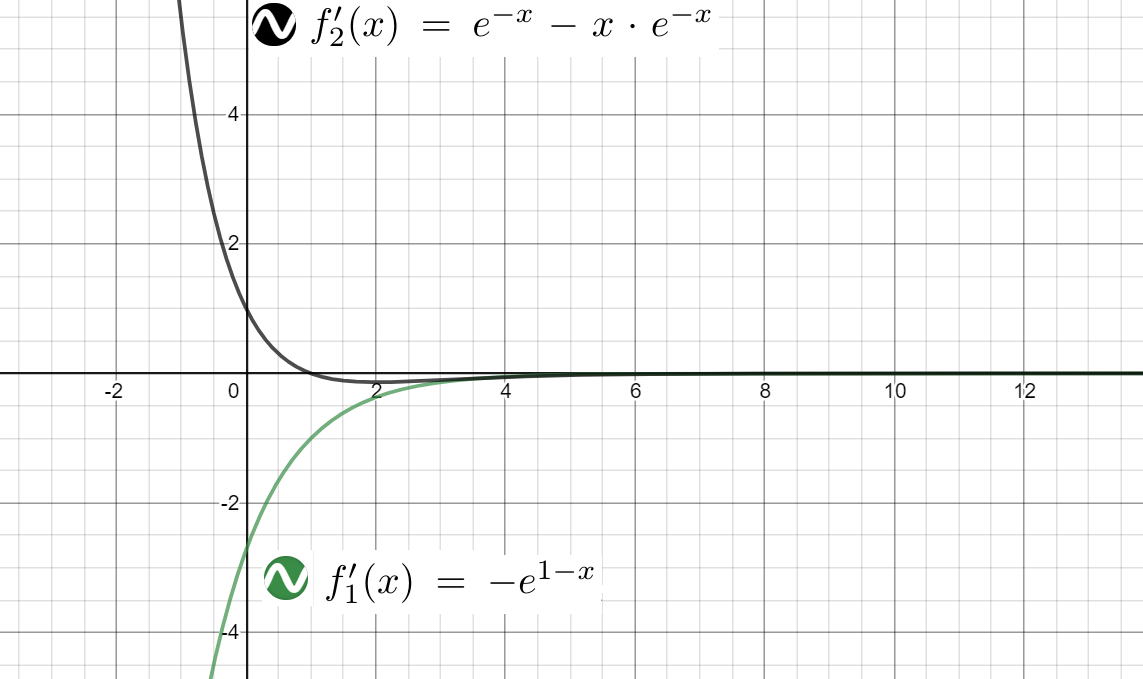
\includegraphics[height=0.39\textheight]{task6derivatives}
		\centering
		\caption{Wykresy pochodnych funkcji $f_1'(x) = -e^{1-x}$, 
			$f_2'(x) = e^{-x} - x\cdot e^{-x}$ narysowane w programie Desmos.}
	\end{figure}

	Przypomnijmy sobie jak działa metoda Newtona gdy trafi na $x_0$ dla którego wartość pochodnej funkcji jest bliska zeru tj. $|f'(x_0)|<\epsilon$. Metoda wtedy zwraca błąd. Widzimy już zatem, że nie możemy wziąć takich wartości x jako przybliżenia początkowe, bo otrzymamy błąd. Dotyczy to obu funkcji, ponieważ obie pochodne mają granicę równą 0 przy $x\to\infty$.\\
	Pozostaje jeszcze inne ważne pytanie, dla jakich $x_0$ metoda Newtona będzie zbieżna? Obliczmy $\phi_1(x) = x - \dfrac{f_1(x)}{f_1'(x)} = x+1-e^{x-1}$ oraz 
	 $\phi_2(x) = x - \dfrac{f_2(x)}{f_2'(x)} = x-\frac{x}{1-x}$. Zobaczmy wykresy oraz punkty stałe odwzorowań $\phi_1(x)$ oraz $\phi_2(x)$. Wykresy poniżej.
	\begin{figure}[!htbp]
		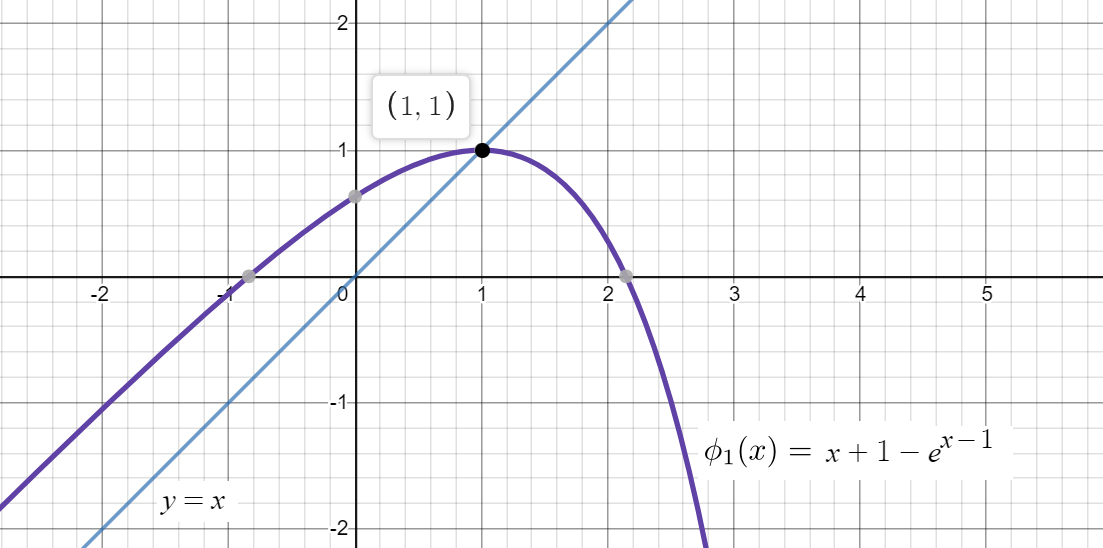
\includegraphics[width=\textwidth]{task6f1phi}
		\centering
		\caption{Wykresy odwzorowania $\phi_1(x) = x+1-e^{x-1}$ oraz prosta $y=x$ narysowane w programie Desmos.}
	\end{figure}
	\begin{figure}[!htbp]
	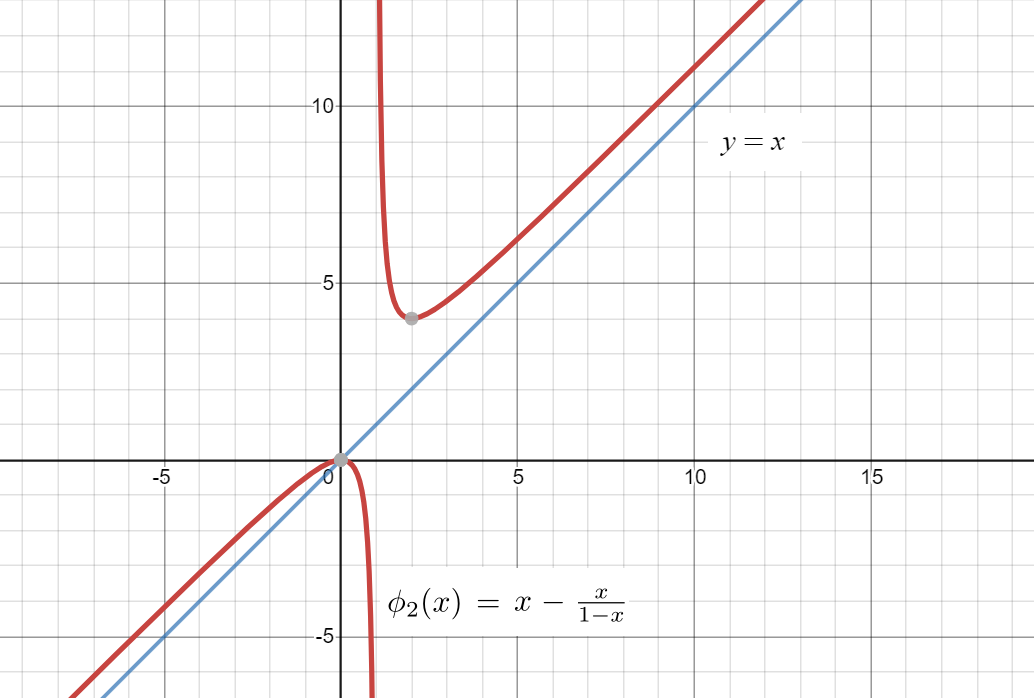
\includegraphics[height=0.40\textheight]{task6f2phi}
	\centering
	\caption{Wykresy odwzorowania $\phi_2(x) = x-\frac{x}{1-x}$ oraz prosta $y=x$ narysowane w programie Desmos.}
	\end{figure}
	
	Po wykresie $\phi_1(x)$ widać, że metoda Newtona dla $f_1$ jest zawsze zbieżna. Zatem jedyną rzeczą jaką musimy uwzględnić przy wybieraniu $x_0$ dla $f_1$ to wyżej wspomniany warunek o wartości pochodnej tj. wartość pochodnej w $x_0$ nie będąca zbyt blisko zera. Zauważmy, że punktem stałym tego odwzorowania jest $x=1$ co pokrywa się z pierwiastkiem.\\
	W treści zadania pojawia się polecenie mówiące żeby sprawdzić co stanie, gdy w metodzie Newtona dla $f_1$ wybierzemy $x_0\in(1,\infty)$. Ogólna odpowiedź to to, że metoda Newtona będzie wtedy zbieżna. Warto jednak dodać, że wynik programu zależy od tego jak duży x wybierzemy. Jeśli weźmiemy na tyle duże $x_0$, że $|f_1'(x_0)|<\epsilon$ to otrzymamy błąd.\\
	Po wykresie $\phi_2(x)$ widać, że metoda Newtona dla $f_2$ nie jest zawsze zbieżna. Dla $x\in(1,\infty)$ metoda Newtona jest rozbieżna, a dla $x\in(-\infty, 1)$ jest zbieżna. Zatem odpowiedzią na pytanie z treści zadania -- co się stanie co stanie, gdy w metodzie Newtona dla $f_2$ wybierzemy $x_0>1$? -- jest to, że wtedy metoda będzie rozbieżna i nigdy nie otrzymamy poprawnego wyniku. Zauważmy też, że punktem stałym odwzorowania $\phi_2(x)$ jest $x=0$ co pokrywa się z pierwiastkiem funkcji $f_2$. Pozostała jeszcze jedna wartość $x_0$ do sprawdzenia, jest to $x_0=1$. W treści zadania również pojawia się pytanie czy można tę wartość wybrać na przybliżenie początkowe.
	Na wykresie $\phi_2(x)$ widać, że w punkcie $x_0 = 1$ przebiega asymptota pionowa. Prościej jednak popatrzeć na wykres $f_2'$. Widać na nim, że $f_2'$ ma w $x_0=1$ miejsce zerowe zatem mamy $f_2'(1) =0$ co w rezultacie daje sytuację, że warunek $|f_2'(x_0)|<\epsilon$ jest spełniony. Powoduje to, że metoda Newtona zwróci błąd. Poniżej rezultaty działania metody Newtona dla wyżej opisanych przypadków.
	\begin{table}[!h]
		\centering
		\label{tab:table1}
		\begin{tabular}{|c|c|c|c|c|}
			\hline
			funkcja & $x_0$ & pierwiastek - $r$ & $f_2(r)$ & liczba potrzebych iteracji\\
			\hline
			$f_1$ & 3.0 & 0.9999999710783241 & 2.892167638712806e-8 & 9\\ \hline
			$f_1$ & 25.0 & \multicolumn{3}{|c|}{błąd - wartość pochodnej funkcji w punkcie $x_0<\epsilon$ } \\ \hline
			$f_2$ & 5.0 & 15.19428398343915 & 3.827247505782987e-6 & 9\\  \hline
			$f_2$ & 1.0 & \multicolumn{3}{|c|}{błąd - wartość pochodnej funkcji w punkcie $x_0<\epsilon$ } \\ \hline
		\end{tabular}
		\caption*{Metoda Newtona dla $f_1$ i $f_2$ dla przypadków szczególnych.}
	\end{table}
	
	\noindent Dla $f_2$ i $x_0=5.0$ otrzymaliśmy błędny wynik, ponieważ metoda Newtona jest wtedy rozbieżna, ale jeden z warunków końca został spełniony, tj. $f_2(x_0) < \epsilon$ -- dlatego metoda zwróciła jakiś wynik.\\
	\textbf{Metoda siecznych}\\
	
	



\end{document}